\documentclass[PlasmaNotes.tex]{subfiles}
\begin{document}
\setcounter{section}{3}
\section{Week 4. Fluid description of plasmas part II, with Paolo Ricci}
\subsection{Single fluid and MHD}
\subsubsection{The two fluid model review}

Each model has:
\begin{itemize}
\item a \textbf{continuity equation}

\[\pd{n_s}{t} + \pd{}{\v{r}} \cdot (n_s \v{u_s} \]

\item A \textbf{momentum equation}

\[ m_s n_s \d{\v{u_s}}{t} = q_s n_s (\v{E} + \crossproduct{u_s}{B}) - \div{\hat{P_s}} + \v{R_s} \]

(where $\d{}{t}$ is the \emph{convective derivative} and $\v{R_s} = \int{m_s (\v{v}-\v{u_s})(\pd{f}{t})_c d\v{v}}$

\item An equation for the pressure - a closure equation, which we won't write here

\item And there's the Maxwell equations to which the fluid model is coupled by

\[ \rho = \sum_s{q_s n_s} \]
\[ \v{j} = \sum_s{q_s n_s \v{u_s}} \]
\end{itemize}

\subsubsection{One-fluid variables}

\begin{itemize}
\item Mass density
\[ \rho_M(\v{r}, t) = \sum_s{n_s m_s} = n_e m_e + n_i m_i \]
\item Center-of-mass velocity
\[ \v{V}(\v{r}, t) = \frac{\sum_s{m_s n_s \v{u_s}}}{\sum_s{n_s m_s}} \]
\item Total electric charge
\[ \rho = \sum_s{n_s q_s} = e(n_i - n_e) \]
\item Total electric current
\[ \v{J} = \sum_s{q_s n_s \v{u_s}} \]
\item Pressure in center of mass frame
\[ \hat{P_s^{cm}} = n_s m_s \int{(\v{v} - \v{V})((\v{v} - \v{V}) f_s d\v{v}} \]
\[ \hat{P^cm} = \sum_s{\hat{P_s^{cm}}} \]
\end{itemize}

\subsubsection{One-fluid equations}

We multiply the continuity equations for both species by their respective masses, add both up and we get
\begin{equation}
\boxed{ \pd{\rho_M}{t} + \pd{}{\v{r} (\rho_M \v{V}) = 0 } }
\end{equation}

Likewise, by multiplying by the species' charge we can get an equation for charge density

\begin{equation}
\boxed{ \pd{\rho}{t} + \pd{}{\v{r}} \cdot \v{J} = 0 }
\end{equation}

Taking the momentum equations and directly summing them to acquire the center of mass velocity equation

\begin{equation}
\boxed{ \rho_M \d{\v{V}}{t} = \rho \v{E} + \crossproduct{j}{B} - \pd{}{\v{r}} \cdot \hat{P^{cM}} }
\end{equation}

Dividing each of the momentum equations by species charge times number density, and also multiplying the ion equation by the ratio $m_e/m_i$ \textbf{and assuming that}
\begin{itemize}
\item $n_e = n_i \equiv n_0$
\item $m_e \ll m_i$
\item current much smaller than current carried by each species

$\v{j} \ll e n \v{u_e}, e n \v{u_i} $
\end{itemize}

We get an \textbf{electron current equation} (also called Ohm's law!)
\begin{equation}
\boxed{ \frac{m_e}{n_e^2} \Big[ \pd{\v{J}}{t} + \pd{}{\v{r}} \cdot ( \v{V} \v{J} + \v{J} \v{V}) \Big] = \v{E} + \crossproduct{V}{B} - \oneover{e n} \pd{}{\v{r}} \hat{P_e^{cm}} - \eta \v{J} }
\end{equation}

\subsubsection{Summary of the one fluid model}

\begin{itemize}
\item Mass continuity equation

\begin{equation}
\boxed{ \pd{rho_M}{t} + \pd{}{\v{r}} (\rho_M \v{V}) = 0 }
\end{equation}

\item Charge continuity equation

\begin{equation}
\boxed{ \pd{\rho}{t} + \pd{}{\v{r}} \cdot \v{J} = 0 }
\end{equation}

\item Momentum equation

\begin{equation}
\boxed{ \rho_M \d{\v{V}}{t} = \rho \v{E} + \crossproduct{j}{B} - \pd{}{\v{r}} \cdot \hat{P^{cM}} }
\end{equation}

\item Ohm's law

\begin{equation}
\boxed{ \frac{m_e}{n_e^2} \Big[ \pd{\v{J}}{t} + \pd{}{\v{r}} \cdot ( \v{V} \v{J} + \v{J} \v{V}) \Big] = \v{E} + \crossproduct{V}{B} - \oneover{e n} \pd{}{\v{r}} \hat{P_e^{cm}} - \eta \v{J} }
\end{equation}

\item Closure, under the assumption of sufficient collisions ($\gamma$ is $1$ for isothermal setting, $\frac{c_P}{c_V}$ for adiabatic, $+\infty$ for incompressible plasmas):

\begin{equation}
\boxed{ \pd{}{\v{r}} \hat{P_{cm}} = \pd{}{\v{r}} P\text{ , } \d{}{t} (P \rho_M^{-\gamma}) }
\end{equation}

\item Maxwell equations

\begin{equation}
\boxed{ \div{E} = \rho/\eps }
\end{equation}
\begin{equation}
\boxed{
\div{B} = 0 }
\end{equation}
\begin{equation}
\boxed{\curl{E} = -\pd{\v{B}}{t} }
\end{equation}
\begin{equation}
\boxed{\curl{B} = \mu_0(\v{j} + \eps \pd{\v{E}}{t}) }
\end{equation}

\end{itemize}

This is a completely closed system of equations! 

\subsubsection{Four simplifying assumptions for the one-fluid model}
\begin{itemize}
\item Negligible electron inertia $m_e \rightarrow 0$. This simplifies Ohm's law to

\[ 0 = \v{E} + \crossproduct{V}{B} - \oneover{e n} \pd{}{\v{r}} \hat{P_e^{cm}} - \eta \v{J} \]

\item Assume quasineutrality ( $L \gg \lambda_D$, $\omega \ll \omega_{pe}, \omega \ll \omega_{ci}$ (ion cyclotron frequency)), $\rho \ll n e$

This lets us neglect Gauss' law, the $\pd{\rho}{t}$ term in the continuity equation and the $\rho \v{E}$ term in the momentum equation

\item Neglect EM waves: $\abs{\eps \pd{\v{E}{t}}{t}} \ll \abs{\v{j}}$

This lets us neglect the displacement current in $\rot{B}$. This implies $\div{j} =0$ and lets us remove the other term in the charge continuity equation

\item Small larmor radius (to neglect finite larmor radius effects): $L \gg \rho_i$, or in other words $\abs{\rot{B}} \gg $, which lets us remove the pressure term in Ohm's law.
\end{itemize}

\begin{center}
\textbf{You have successfully crafted a $+3$ Magnetohydrodynamics Model of Quality!}
\end{center}

\subsubsection{The MHD model}
\begin{itemize}
\item Continuity equation (for mass density)
\begin{equation}
\boxed{ \pd{\rho_M}{t} + \pd{}{\v{r}}(\rho_M \v{V})}
\end{equation}
\item Momentum equation

\begin{equation}
\boxed{ \rho_M \d{\v{V}}{t} = \crossproduct{J}{B} - \pd{P}{\v{r}} }
\end{equation}
\item Ohm's law

\begin{equation}
\boxed{ \v{E} + \rot{B} = \eta \v{J} }
\end{equation}

\item Closure (pressure, TD) equation
\begin{equation}
\boxed{ \d{}{t} (P \rho_M^{-\gamma})=0 }
\end{equation}

\item Maxwell equations
\begin{equation}
\boxed{  \rot{E} = -\pd{\v{B}}{t} }
\end{equation}
\begin{equation}
\boxed{ \rot{B} = \mu_0 \v{J} }
\end{equation}
\begin{equation}
\boxed{ \div{B} = 0 }
\end{equation}
The last one is an initial condition for B.
\end{itemize}

This is a system of $14$ equations in $14$ unknowns $\rho_M$, $\v{V}$, $\v{J}$, $\v{B}$, $P$, $\v{E}$.

For sufficiently hot temperatures, the resistivity $\eta$ can be neglected for the \emph{ideal MHD model}. If not, it's a \emph{resistive MHD model}.

\subsubsection{MHD simulations}

Good for global dynamics of a plasma, especially for fusion plasma confinement devices. Example - W7-X MHD simulation done by EPFL group - equilibrium magnetic field.




\subsection{MHD equilibrium and applications in one dimension}

\subsubsection{Static ideal MHD equilibria}
The MHD equations are
\[ \pd{\rho_M}{t} + \pd{}{\v{r}}(\rho_M \v{V}) \]
\[ \rho_M \d{\v{V}}{t} = \crossproduct{J}{B} - \pd{P}{\v{r}} \]
\[ \v{E} + \rot{B} = \eta \v{J} \={\text{for ideal MHD } \eta = 0} 0 \]
\begin{center}
\end{center}
\[ \d{}{t} (P \rho_M^{-\gamma})=0 \]
\[\rot{E} = -\pd{\v{B}}{t} \]
\[ \rot{B} = \mu_0 \v{J} \]
\[ \div{B} = 0 \]

In a static equilibrium, $\pd{}{t} =0$. We'll also focus on $\v{V}=0$. Transforming the equations, the continuity equation, the $\curl{E}$ Maxwell equation and the closure equation drop out. The momentum equation becomes the force balance equation
\[ 0 = \crossproduct{J}{B} - \pd{P}{\v{r}} \]
From Ohm's law
\[ \v{E} = 0 \]
\[ \rot{B} = \mu_0 \v{J} \]
\[ \div{B} = 0 \]

These four equations give the conditions for static equilibrium in ideal MHD.

\subsubsection{Force balance equation analysis}
If we dot $\dotproduct{B}{\grad{P}} = \dotproduct{B}{(\crossproduct{j}{B})} \={\perp} 0$. Likewise, $\dotproduct{j}{\grad{P}} = \dotproduct{j}{(\crossproduct{j}{B})} \={\perp} 0$. Thus, both the magnetic field lines and current run along isobaric (constant pressure) surfaces.

Substituting $\curl{B}$ into the force balance equation, we get
$\oneover{\mu_0} \crossproduct{(\rot{B})}{B} \sim \frac{B^2}{mu_0 l} = \grad{P} \sim \frac{P}{l}$, where $l$ is a characteristic length.

We define
\begin{equation}
\boxed{\beta = \frac{P}{(\frac{B^2}{2\mu_0})} \ll 1 }
\end{equation}
The condition $\beta \ll 1$ is fulfilled for a typical lab plasma. For high $\beta$, the plasma's kinetic energy is much higher than the energy in its magnetic field. For the Earth's magnetosphere, $\beta \sim 1$. In some astrophysical systems, $\beta$ can be larger than $1$.

\begin{equation}
\boxed{\crossproduct{(\rot{B})}{B} = 0}
\end{equation}
This is called the \textbf{force free equilibrium}, for very low $\beta$. For higher $\beta$, we get the \textbf{force balance equilibrium}

\begin{equation}
\boxed{\oneover{\mu_0}\crossproduct{(\rot{B})}{B} = \grad{P}}
\end{equation}

\subsubsection{Force-free equilibria}

One example of force free equilibrium is the surface of the sun. Since the curl of B is parallel to B itself,
\[\curl{B} = \alpha \v{B} \]
\[\div{(\alpha B)} = \dotproduct{B}{\grad{\alpha}} = 0 \]

This means that B runs along surfaces of constant $\alpha$.

For cylindrically symmetric situations ($\vartheta$ symmetry), $\curl{B} = \alpha \v{B}$ is satisfied by

\begin{equation}
\boxed{v{B} = B_{\vartheta} \uv{\vartheta} + B_z \uv{z} = \frac{B_0 K r}{1+k^2 r^2} \uv{\vartheta} + \frac{B_0}{1+k^2 r^2} \uv{z} }
\end{equation}


This gives
\[\alpha = \frac{\mu_0 j_z}{B_z}\]

\[j_z = \frac{2 k B_0/\mu_0}{(1+k^2 r^2)^2}\]


$K$ is a $1/m$ constant that sets the scale of the equilibrium. $r$ is the radial distance.

We imagine nested cylinders of decreasing radius. The $B$ field runs along their surfaces. At small $r$, B is mostly along $\uv{z}$. At higher radii, $B$ is along $\uv{\vartheta}$. This is a so called \textbf{flux rope}. These are the flumes on the surface of the sun!

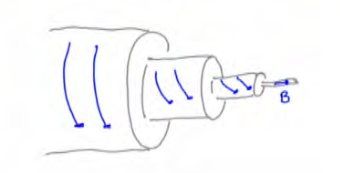
\includegraphics{fluxrope}

\subsubsection{Force-balanced equilibria}

We plug in
\[\crossproduct{(\rot{B})}{B} = \crossproduct{(\dotproduct{B}{\nabla})}{B} - \frac{1}{2} \nabla B^2 \]

Which gives us

\begin{equation}
\boxed{ \grad{(P + \frac{B^2}{2\mu_0})} = \oneover{\mu_0} (\dotproduct{B}{\nabla}) \v{B} }
\end{equation}

The terms above are the so called plasma pressure, magnetic pressure and field line tension.

\subsubsection{Force-free and force-balanced equilibria}

For a cylindrical symmetry as before, and pressure and magnetic field components depending only on radial distance

\[ \d{}{r} \Big(P + \frac{B_{\vartheta}^2+B_z^2}{2\mu_0}\Big) = - \frac{B_{\vartheta}^2}{\mu_0 r} \]

This allows us to get the current, as $\v{j} = \oneover{\mu_0} \grad{B}$:

\[\v{j} = j_{\vartheta} \uv{\vartheta} + j_z \uv{z} = -\oneover{\mu_0} \d{B_z}{z} + \oneover{\mu_0 r} \d{}{r}(r B_{\vartheta}) \]

Two of these functions - $B_{\vartheta}, B_z, P$ (all depending on $r$) can be specified arbitrarily, the third will get determined by the relations above and boundary conditions. 

\subsubsection{Z pinch, theta pinch}

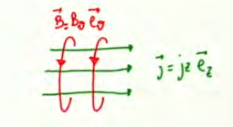
\includegraphics{zpinch}

The Z, or Bennett pinch has $B_z=0$. The plasma is confined by the $\uv{\vartheta}$ magnetic field. The current runs in the z direction.

One example is a uniform current running through a plasma:

\[ j_z = j_{z0} \text{ for } r\leq a \text{ and beyond that } 0 \]

\[I = \int_0^a{j_z 2 \pi r dr} = \pi a^2 j_{z0} \]

This implies

\[ B_{\vartheta} = \frac{\mu_0 I r}{2 \pi a^2} \]
and outside the plasma
\[ B_{\vartheta} = \frac{\mu_0 I}{2 \pi r} \]

We can write the force balance equation

\[ \d{}{r} \Big(P + \frac{B_{\vartheta}^2}{2\mu_0} \Big) = - \frac{B_{\vartheta}^2}{\mu_0 r} \]

And from the condition that outside the plasma, its pressure is zero, we get

\[ P(r) = \mu_0 (\frac{I}{2 \pi a})^2 (1-\frac{r^2}{a^2}) \]

There's also the theta $\vartheta$ pinch:

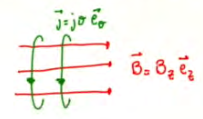
\includegraphics{thetapinch}


For which the force balance equation is very simple:

\[\d{(P+\frac{B_z^2}{2\mu_0})}{z}=0 \]

\subsection{MHD stability, with Duccio Testa}
\subsubsection{What if a MHD equilibrium plasma is perturbed?}
Different kinds of instabilities from CM:

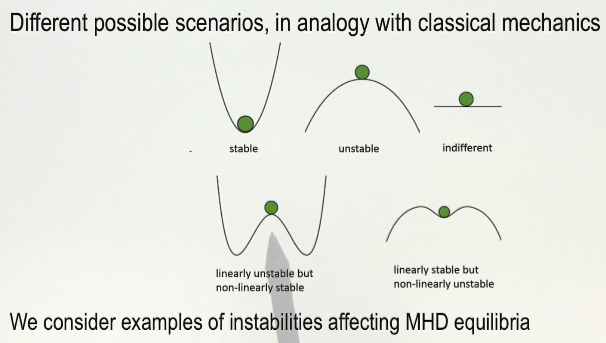
\includegraphics{mhdclassicalmechanicsinstabilities}

What we're interested in is unstable equilibria.

We first examine the wonderfully named \textbf{sausage instability}. In a Z-pinch (axial current, azimuthal B field), the balance is between the magnetic field lines' tension, the gradient of the pressure, and the magnetic field itself ($B_{\vartheta}^2$ term).

At a compression point, the radius of the cross section is smaller; $B_{\vartheta}$ increases, the pressure also increases and this squeezes the plasma.

Likewise, at a bulge, B decreases, the pressure decreases and the plasma tends to expand.

\textbf{Kink instabilities} form when Z-pinches are bent; at the point of negative curvature, field lines come closer together, the B field increases, the pressure increases and the plasma is pushed towards having even more curvature.

\textbf{Rayleigh-Taylor instabilities}. Assume a plasma above a region of vacuum (or air), with a small ripple at the boundary. The $\crossproduct{g}{B}$ drift will separate electrons and ions. There's a charge separation and a resulting E field. A $\crossproduct{E}{B}$ drift at the ripples will tend to magnify them, leading to instability.

This is just like in fluids!

Consider the curvature drift $F_c \sim \v{R_c}$. If the B field surrounds a plasma (concave towards plasma), the drift will magnify the instability. Otherwise, it will bring the plasma towards equilibrium (`good curvature').

\subsubsection{Wall effect on MHD instabilities}

Axial current, azimuthal B field. Plasma surrounded by ideal (no resistivity) wall which - we assume - it cannot penetrate.

We consider the conservation of magnetic flux $\Phi = \int_S{B \cdot dS}$.
\[ \d{\Phi}{t} = \int_S{\pd{B}{t} \cdot dS} + \int_S{B \cdot dS} \]

Plug in Faraday's law and Stokes' theorem, we get

\[ \int_S{\pd{B}{t} \cdot dS } = - \oint_C{E \cdot dL} \]

\[ \int_S{B \cdot \d{}{t} dS} = \oint_C{\dotproduct{B}{\crossproduct{V}{dl}}}\]

Summing up the two terms and using a vector identity, we actually get Ohm's law. But since we're in ideal MHD, the integrand is zero! The magnetic flux is indeed constant.

The magnetic field is compressed at the plasma-wall boundary. B increases, P increases and pushes the plasma back towards the center. Surround a plasma with a wall and it gets stabilized! However, in practice the wall's resistivity is finite and it is only stabilised for some time.

\subsubsection{General methods for MHD stability analysis}

For uniform plasmas - use fourier mode analysis and if $Im(\omega)>0$, we get exponential perturbation growth and instability.

For non-uniform plasmas - fourier analysis in time for Newton's law in fluid displacement gives a harmonic oscillator equation where the sign of $\omega^2$ determines stability. Can also do energy analysis:

This is the change in potential energy. Sign determines stability.

\subsubsection{MHD instability control}
Passive methods, such as walls. Active control - when we notice an instability begins to grow, we use active feedback (lithium? magnetic resonance for ELMs?).

\subsection{MHD waves}
The handouts have gotten amazing so I will be doing less transcription of equations and more commentary now.

Plasma waves in the MHD model include: shear Alfven waves, fast compressional Alfven waves and slow magnetosonic waves. It's the same old story - use ideal MHD equations, add small perturbations, linearize about the equilibrium, fourier transform, look at frequencies and see whether they suggest exponential growth.

The sound speed squared depends on the equilibrium value of pressure.

We're working on a set of 4 equations.

To pick a geometry, we choose a wave propagating in the $XZ$ plane and a B field along the Z axis. We can have either transverse waves - velocity oscillates in the $Y$ direction - or longitudinal waves - along $k$ in the $XZ$ plane.

\subsubsection{Transverse - shear Alfven - waves}

Transverse waves are not compressible ($\rho_{M1} =0$)!

Nontrivial solutions give the shear alfven wave dispersion relation using 

\[ \omega^2 = k_z^2 c_A^2 = k^2 c_A^2 \cos{\theta}^2 \]

These are important in DT fusion plasmas. Velocity of $\alpha$ particles at $E=3.5 MeV$ is greater than $c_A$, they're said to be superAlfvenic and they become resonant. Whatever that means.

\subsubsection{Longitudinal - fast compressional Alfven - waves}

Redoing all the earlier calculation and neglecting terms of high order in the $\frac{c_S^2}{c_A^2}$ ratio, we get two ($\pm$) solutions. Denote $\omega_+$ as the solution to the $+$ equation. Neglecting high order terms once more, we get

\[ \omega_+^2 = k^2 c_A^2 (1+\frac{c_S^2}{c_A^2} \sin{\theta}^2) \]

This is called the fast compressional Alfven wave - fast in phase velocity, relative to sound speed. The sound speed in fact only enters as a small correction.

Taking the $-$ solution we get the slow magneto-sonic wave

\[ \omega_-^2 = k^2 c_S^2 \cos{\theta}^2 \]

\end{document}